\section{Game Theoretic approach to Tree-Depth}

\subsection{Defining the game}
\paragraph{}
The k-step selection-deletion game is played by Alice and Bob on a graph. The game is played by turns as follows:
\begin{itemize}
  \item First, Alice selects a connected component of the graph, and the rest of the components are deleted.
  \item Then, Bob deletes a node from the remaining graph and the next round is played with this graph.
\end{itemize}

If Bob deletes the last node at the k-th round or earlier, he is said to win the k-step selection-deletion game. Otherwise, Alice wins.
\paragraph{}
From this definition we can observe that if Bob has a strategy to win in k rounds that strategy will also guaranty a win in any game that lasts more than k rounds. Conversely, if Alice has a winning strategy in k-rounds, that same strategy will also win any game with less than k rounds.

\subsection{Bob's winning strategy}
\begin{lemma}
Let G be a graph and let F be a rooted forest of height t such that G $\subseteq$ clos(F). Then, Bob has a winning strategy for the (t+1)-step selection-deletion game.
\label{lemma:Bob-win}
\end{lemma}
\begin{proof}
Because of lemma~\ref{lema:min-ET} we know an elimination forest Y exists such that height(Y) $\leq$ height(F).
Consider h = height(Y), we will proof that Y encodes a winning strategy in h+1 rounds which is also a winning strategy in the t+1-step selection-deletion game because h $\leq$ t.
\begin{itemize}
  \item \textbf{Base case}: If h = 0, then every component of G will have a single vertex, so it's clear that Bob will win the 1-step selection-deletion game.
  \item \textbf{Induction}: Let $G_i \subseteq G$ be the component Alice chooses, then $Y_i$ exists such that $Y_i$ is an elimination tree belonging to Y, $G_i \subseteq clos(Y_i)$ and obviously $height(Y_i) \leq h$. Bob will delete v, the root of $Y_i$. This will leave us with $G' = G_i - v$ as the new graph. If we consider the children of v the new roots in $Y' = Y_i - v$, then $G' \subseteq clos(Y')$ because of how the elimination trees are built. As $height(Y') \leq h-1$, we can assume by induction that Bob has a winning strategy in h rounds for $G'$, which together with the strategy for the first round we have just defined makes a winning strategy for Bob in the (h+1)-step selection-deletion game on the graph G.
\end{itemize}
\end{proof}

\subsection{Alice's winning strategy}
\begin{definition}
A shelter S in a graph G is a partially ordered set of graphs with the next properties:
\begin{itemize}
  \item $\forall H \in S$, $H \subseteq G$ and $H$ is connected.
  \item $H \leq M$ if and only if $H \subseteq M$.
  \item If $H \in S$ and $H$ is not minimal, then $\forall v \in V(H)$, there exists $H' \subseteq H - v$ such that $H$ covers $H'$. In a partially ordered set $a$ covers $b$ means that $a \neq b$, $a \geq b$, and no c exists such that $c \neq a \neq b$ and $a \geq c \geq b$.
\end{itemize}
\end{definition}

\begin{figure}[H]
\usetikzlibrary{arrows}
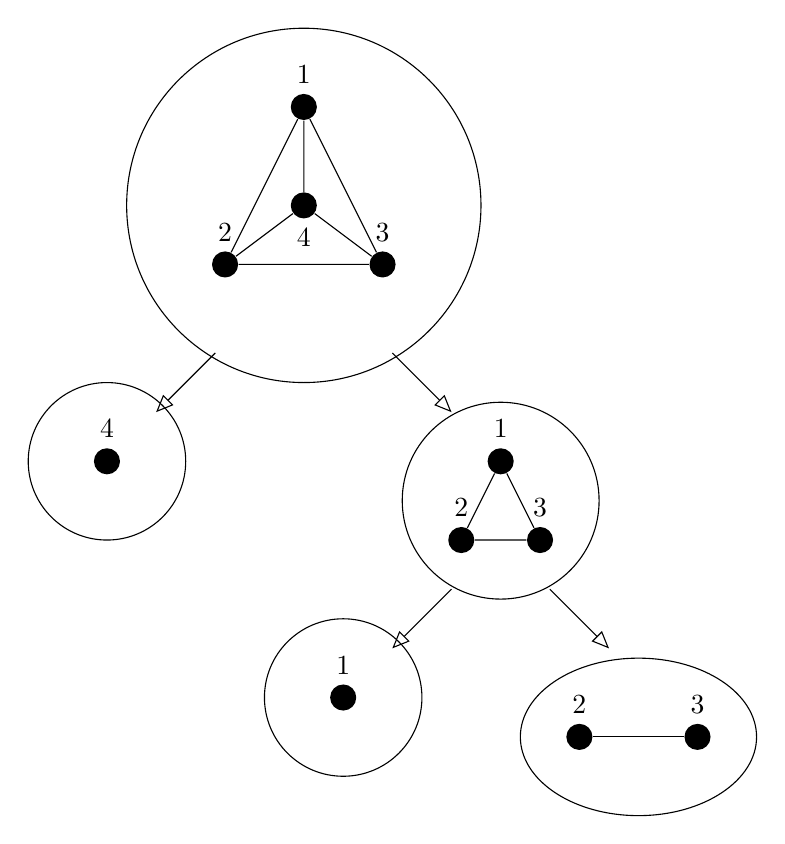
\begin{tikzpicture}





\node [fill, circle, label=1] (v2) at (-1.5,4) {};

\node [fill, circle, label=2] (v1) at (-2.5,2) {};

\node [fill, circle, label=3] (v3) at (-0.5,2) {};

\node [fill, circle, label=below:4] (v4) at (-1.5,2.75) {};

\draw (v1) -- (v2) -- (v3) -- (v1) -- (v4) -- (v2);

\draw  (v4) edge (v3);

\draw  (v4) ellipse (2.25 and 2.25);

\node (v5) at (-2.5,1) {};

\node (v6) at (-3.5,0) {};

\node (v7) at (-0.5,1) {};

\node (v8) at (0.5,0) {};

\draw [-open triangle 45] (v5) edge (v6);

\draw [-open triangle 45] (v7) edge (v8);



\node [fill, circle, label=4] (v9) at (-4,-0.5) {};



\draw  (v9) ellipse (1 and 1);

\node [fill, circle, label=1] (v10) at (1,-0.5) {};

\node [fill, circle, label=2] (v12) at (0.5,-1.5) {};

\node [fill, circle, label=3] (v11) at (1.5,-1.5) {};

\draw (v10) -- (v11) -- (v12) -- (v10);

\draw  (1,-1) ellipse (1.25 and 1.25);

\node (v13) at (0.5,-2) {};

\node (v15) at (1.5,-2) {};

\node (v14) at (-0.5,-3) {};

\node (v16) at (2.5,-3) {};

\draw [-open triangle 45] (v13) edge (v14);

\draw [-open triangle 45] (v15) edge (v16);

\node [fill, circle, label=1] (v17) at (-1,-3.5) {};
\draw  (v17) ellipse (1 and 1);




\node [fill, circle, label=2] (v18) at (2,-4) {};

\node [fill, circle, label=3] (v19) at (3.5,-4) {};

\draw  (2.75,-4) ellipse (1.5 and 1);

\draw  (v18) edge (v19);

\end{tikzpicture}
\caption{An example of a shelter. The arrows represent the covering relation. \label{fig:shelter-example}}
\end{figure}
The thickness of a shelter S is the shortest chain from a maximal element in S to a minimal element in S. The length of a chain is defined as the number of elements in it minus one. The thickness of the shelter in figure~\ref{fig:shelter-example} is 1, because of the chain $\left\{ 1, 2, 3, 4\right\} \geq \left\{4\right\}$.
\begin{lemma}
Let G be a graph, S a shelter in G, and t the thickness of S. Then, S encodes a winning strategy for Alice in the t-step selection-deletion game.
\label{lemma:Alice-win}
\end{lemma}
\begin{proof}
We will proof this by induction over t.
\begin{itemize}
  \item \textbf{Base case}: If t = 0, then clearly Alice wins the 0-step selection-deletion game.
  \item \textbf{Induction}: Let H be a maximal element in S. Then, Alice picks the connected component $G_i$ of $G$, such that $H \subseteq G_i$. Because t $>$ 0, H is not minimal, so for any vertex $v$ that Bob removes, if $v \in H$ there exists $H' \in S$ that is covered by H and $v \notin H'$. Otherwise, $H$ is still a subgraph of $G_i - v$. Let $S' =\left\{X \mid X \in S \, and \, X \subseteq G_i - v\right\}$. It is clear that $S'$ is a shelter for $G_i - v$ and that the thickness of $S'$ is greater than or equal to t-1. By induction we can assume $S'$ encodes a winning strategy in t-1 steps, which together with the strategy for the first round we have just defined is a winning strategy for the t-step selection-deletion game.
\end{itemize}
\end{proof}


\subsection{Relation to Tree-Depth}

\paragraph{}
It is clear that if Alice has a winning strategy in the t-step selection deletion game, Bob can't have a winning strategy in that same game. Because of this and lemmas~\ref{lemma:Bob-win} and ~\ref{lemma:Alice-win} we can state the following:
\begin{theorem}
Let G be a graph, S a shelter in G of thickness x and F a rooted forest of height y such that G $\subseteq$ clos(F). Then the following is true.
\begin{enumerate}
\item Alice has a winning strategy in the t-step selection-deletion game, for any t smaller than or equal to x.
\item Bob has a winning strategy in the (t+1)-step selection-deletion game, for any t greater than or equal to y.
\item Every rooted forest who's closure contains G has an height higher than or equal to x. Otherwise, Bob would have a winning strategy in the x-step selection-deletion game, which contradicts statement 1.
\item Every shelter in G has a thickness smaller than or equal to y. Otherwise, Alice would have a winning strategy in the (y+1)-step selection-deletion game, which contradicts statement 2.
\item Because we have F, $td(G) \leq y$. Also, from statement 3 it is clear that $x \leq td(G)$. So we can say that $x \leq td(G) \leq y$.
\end{enumerate}
\end{theorem}

\paragraph{}
With this theorem we can now give an upper-bound and a lower-bound to a graphs tree depth.

\begin{figure}[H]
\usetikzlibrary{arrows}
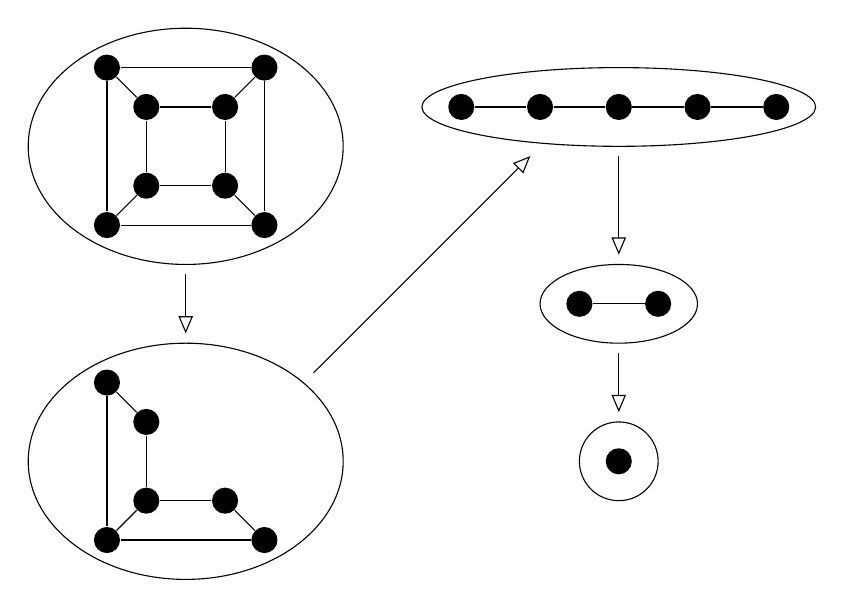
\begin{tikzpicture}
 
\node [circle, fill] (v3) at (-2.5,2.5) {};
\node [circle, fill] (v2) at (-4.5,2.5) {};
\node [circle, fill] (v1) at (-4.5,4.5) {};
\node [circle, fill] (v4) at (-2.5,4.5) {};
\node [circle, fill] (v5) at (-4,4) {};
\node [circle, fill] (v8) at (-3,4) {};
\node [circle, fill] (v6) at (-4,3) {};
\node [circle, fill] (v7) at (-3,3) {};
\node [circle, fill] (v10) at (-4.5,0.5) {};
 
 
\node [circle, fill] (v9) at (-4,0) {};
\node [circle, fill] (v12) at (-4,-1) {};
\node [circle, fill] (v11) at (-4.5,-1.5) {};
\node [circle, fill] (v13) at (-3,-1) {};
\node [circle, fill] (v14) at (-2.5,-1.5) {};
 
\node [circle, fill] (v16) at (0,4) {};
\node [circle, fill] (v17) at (1,4) {};
\node [circle, fill] (v18) at (2,4) {};
\node [circle, fill] (v19) at (3,4) {};
 
 
\draw  (-3.5,-0.5) ellipse (2 and 1.5);
\draw  (-3.5,3.5) ellipse (2 and 1.5);
 
\node [circle, fill] (v15) at (4,4) {};
\draw  (v18) ellipse (2.5 and 0.5);
 
\node [circle, fill] (v30) at (1.5,1.5) {};
\node [circle, fill] (v29) at (2.5,1.5) {};
\node [circle, fill] (v20) at (2,-0.5) {};
\draw  (2,1.5) ellipse (1 and 0.5);
\draw  (v20) ellipse (0.5 and 0.5);
\node (v21) at (-3.5,2) {};
\node (v22) at (-3.5,1) {};
\node (v23) at (-2,0.5) {};
\node (v24) at (1,3.5) {};
\node (v25) at (2,3.5) {};
\node (v26) at (2,2) {};
\node (v27) at (2,1) {};
\node (v28) at (2,0) {};
\draw [-open triangle 45] (v21) edge (v22);
\draw [-open triangle 45] (v23) edge (v24);
\draw [-open triangle 45] (v25) edge (v26);
\draw [-open triangle 45] (v27) edge (v28);
\draw  (v1) edge (v5);
\draw  (v5) edge (v6);
\draw  (v6) edge (v2);
\draw  (v2) edge (v1);
\draw  (v1) edge (v4);
\draw  (v4) edge (v8);
\draw  (v8) edge (v5);
\draw  (v6) edge (v7);
\draw  (v7) edge (v8);
\draw  (v3) edge (v7);
\draw  (v2) edge (v3);
\draw  (v4) edge (v3);
\draw  (v16) edge (v17);
\draw  (v18) edge (v17);
\draw  (v19) edge (v18);
\draw  (v19) edge (v15);
\draw  (v29) edge (v30);
\draw  (v10) edge (v11);
\draw  (v9) edge (v12);
\draw  (v14) edge (v11);
\draw  (v10) edge (v9);
\draw  (v13) edge (v12);
\draw  (v14) edge (v13);
\draw  (v12) edge (v11);
\end{tikzpicture}
\caption{This is a shelter of thickness 4 for the graph in Figure~\ref{fig:3d-cube}. Beware that not all graphs in the shelter are drawn, but every graph in the shelter is isomorphic to these. With this and the rooted forest from Figure~\ref{fig:3d-cube} we can say that td(G) = 4. 
\label{fig:3d-cube-shelter}}
\end{figure}